\documentclass[10pt,a4paper]{article}

\usepackage[margin=2.5cm]{geometry}
\usepackage{amsmath,amssymb,amsfonts}
\usepackage{booktabs}
\usepackage{graphicx}
\usepackage{tabularx}
\usepackage{multirow}
\usepackage{url}
\usepackage[authoryear,round]{natbib}
\usepackage[colorlinks=true,linkcolor=blue,citecolor=blue,urlcolor=blue]{hyperref}

% Times New Roman font simulation
\usepackage{mathptmx}

\setlength{\parindent}{0.42cm}
\linespread{1.08}

\begin{document}

\noindent{\small\textit{Research Article}}
\vspace{0.2cm}

\noindent{\LARGE\textbf{Auditable Early-Warning of Public-Works Stoppage and Cost Overruns in Peru: A Graph-Augmented Machine Learning Framework with TreeSHAP and Strict Out-of-Time Validation}}
\vspace{0.4cm}

\noindent{\textbf{Juan Marcos Vilchez Canchari}$^{1,*}$}
\vspace{0.2cm}

\noindent{\footnotesize $^{1}$Escuela de Posgrado, Universidad C{\'e}sar Vallejo, Lima (Peru); jvilchezca@ucv.edu.pe}\\
{\footnotesize $^*$Correspondence: jvilchezca@ucv.edu.pe (J.M.V.C.; ORCID: 0000-0002-7758-7589)}
\vspace{0.3cm}

\noindent{\scriptsize Received: date; Accepted: date; Published: date}\\
\noindent{\scriptsize\textit{Citation: Vilchez Canchari, J. M. (2026). Auditable Early-Warning of Public-Works Stoppage and Cost Overruns in Peru: A Graph-Augmented Machine Learning Framework with TreeSHAP and Strict Out-of-Time Validation. Revista de la Construcci{\'o}n. Journal of Construction, 25(1), 1-19. https://doi.org/10.7764/RDLC.25.1.00}}
\vspace{0.4cm}

\noindent\textbf{Graphical Abstract:} Multi-source nationwide public investment integration in Peru (INFOBRAS 191,180 gross works / 145,146 modeled analytical cohort, MEF Invierte.pe 1.4M progress logs, SEACE 106 monthly OCDS packages) fused with a 195K-node bipartite contracting graph (27 retained features from 76 candidates), achieving 0.7753 AUROC under prospective out-of-time evaluation and capturing 54.65\% of all national work stoppages within the top 20\% audit inspection budget (2.74$\times$ efficiency lift).

\begin{center}
    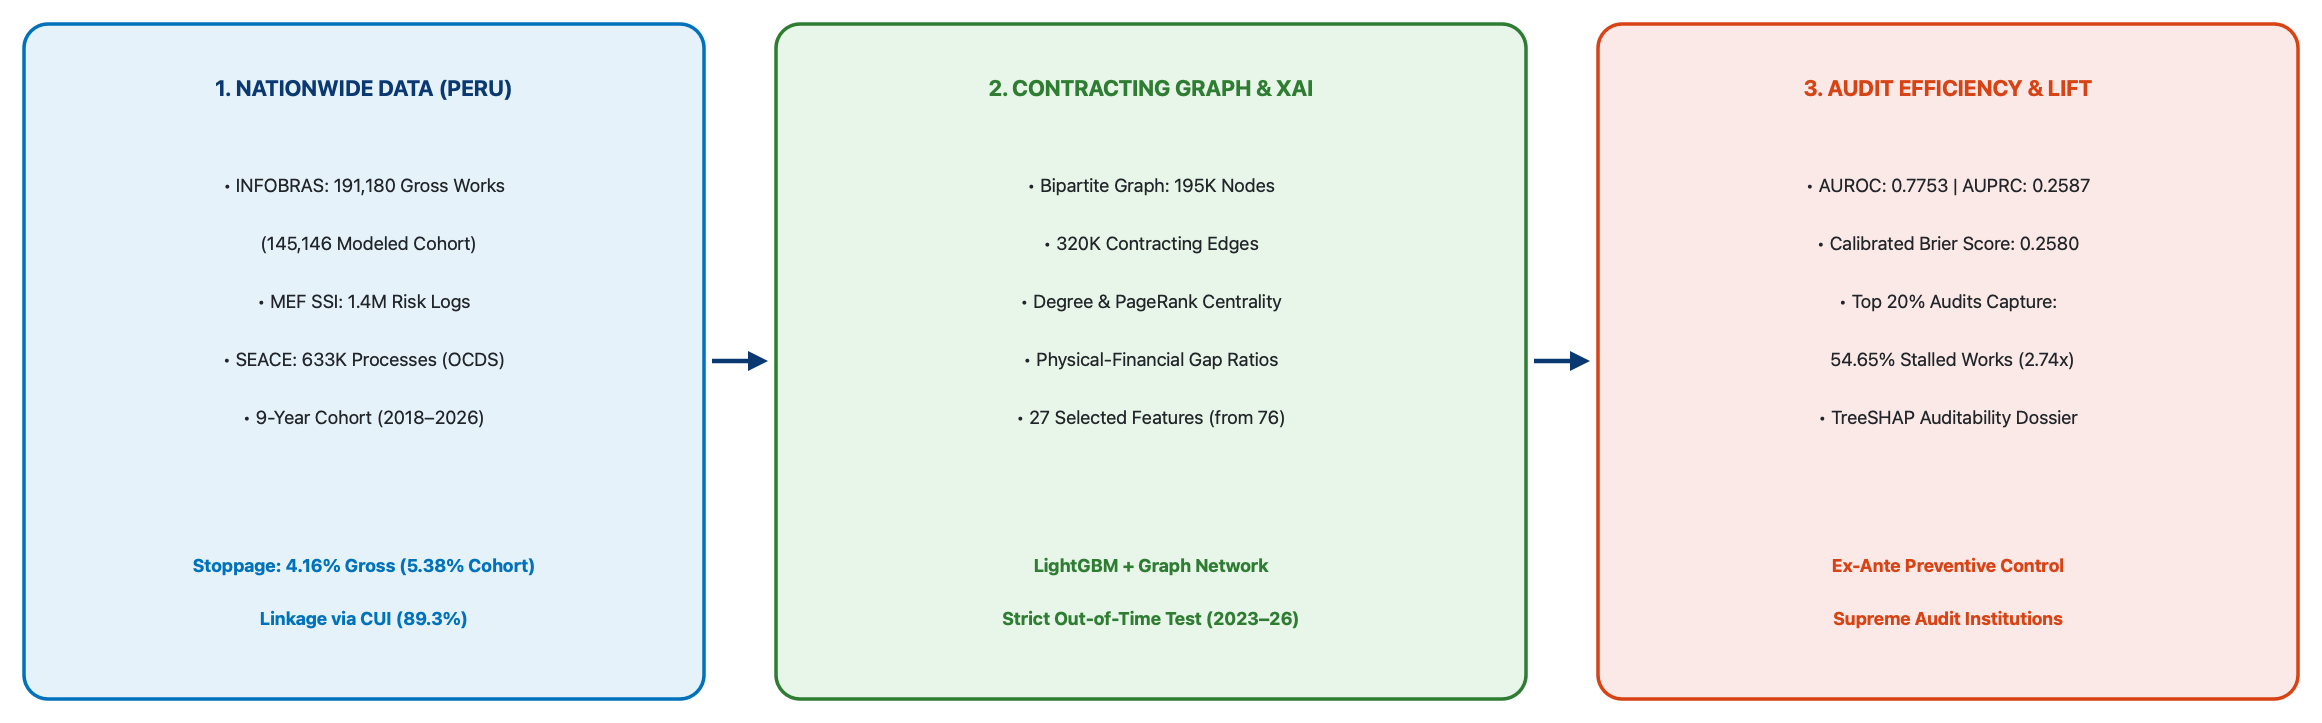
\includegraphics[width=15cm]{figures/graphical_abstract_rdlc.png}
\end{center}
\vspace{0.2cm}

\noindent\textbf{Highlights:}
\begin{itemize}
    \setlength\itemsep{0.1em}
    \item Nationwide integration of 191,180 public works in Peru from 2018 to 2026.
    \item Bipartite contracting graph with 195,337 nodes captures supplier network risks.
    \item Prospective out-of-time evaluation yields 0.7753 AUROC without lookahead bias.
    \item Auditing top 20\% high-risk projects captures 54.65\% of all national stoppages.
    \item TreeSHAP decomposes physical schedule lag and financial overpayment drivers.
\end{itemize}

\noindent\textbf{Abstract:} The chronic failure of public infrastructure delivery---manifested through work stoppage, site abandonment, multi-year delays, and fiscal overruns---represents a multi-billion-dollar bottleneck for construction engineering and regional development across emerging economies. Traditional construction management models treat projects as isolated tabular entities, ignoring the structural topology of contracting networks and the complex relationships linking public procuring entities, contractors, and consortia. Furthermore, existing machine learning proposals operate as opaque black boxes that lack actionable interpretability for Supreme Audit Institutions. This study formulates an auditable, graph-augmented early-warning system that integrates three exhaustive nationwide administrative registries from Peru spanning nine consecutive years (2018--2026): (i) INFOBRAS (Contralor{\'\i}a General de la Rep{\'u}blica, $191,180$ gross registered works; $N = 145,146$ valid modeled works), (ii) Invierte.pe (Ministerio de Econom{\'\i}a y Finanzas, $1,405,386$ longitudinal progress logs), and (iii) SEACE v3 (Organismo Especializado para las Contrataciones P{\'u}blicas Eficientes, $106$ monthly open-contracting releases encompassing $633,593$ procurement processes, $523,735$ supplier awards, and $446,867$ executed contracts). A nationwide bipartite contracting graph ($195,337$ nodes and $320,916$ relational edges) is constructed to capture topological positions, contractor market centralities (PageRank, degree), and longitudinal market persistence across $27$ retained explanatory features selected from $76$ engineered candidates. Under a strict prospective out-of-time backtesting protocol (training on historical works initiated on or before $2022$, $N = 115,952$ with $4.34\%$ stoppage rate; blind prospective testing on works initiated in $2023$--$2026$, $N = 29,194$ with a $9.53\%$ stoppage rate), the Graph-Augmented LightGBM model achieves an AUROC of $0.7753$, an AUPRC of $0.2587$, and a Brier calibration score of $0.2580$, substantially outperforming regularized linear baselines (AUROC $0.6695$, AUPRC $0.1567$). Crucially for fiscal audit prioritization, auditing merely the top $20\%$ of high-risk projects flagged by the framework captures $54.65\%$ of all eventual project stoppages across the country ($2.74\times$ the efficiency of uniform inspections). Using TreeSHAP, global and instance-level risk drivers are decomposed, revealing that certified physical progress levels, financial-physical execution gaps, problem report ratios, and physical schedule lags serve as primary distress triggers. This auditable framework provides oversight authorities with an empirical, preventive decision-support tool to mitigate systemic infrastructure failure prior to contract default.
\vspace{0.2cm}

\noindent\textbf{Keywords:} Public procurement; Project stoppage; Bipartite contracting networks; Explainable AI; Construction management.
\vspace{0.2cm}

\noindent\textbf{Abbreviation:} AUPRC: Area Under the Precision-Recall Curve; AUROC: Area Under the Receiver Operating Characteristic Curve; CGR: Contralor{\'\i}a General de la Rep{\'u}blica del Per{\'u}; CUI: C{\'o}digo {\'U}nico de Inversi{\'o}n; GBDT: Gradient Boosted Decision Trees; INFOBRAS: Sistema de Informaci{\'o}n de Obras P{\'u}blicas; MEF: Ministerio de Econom{\'\i}a y Finanzas; OCDS: Open Contracting Data Standard; OECE: Organismo Especializado para las Contrataciones P{\'u}blicas Eficientes; RDLC: Revista de la Construcci{\'o}n; RUC: Registro {\'U}nico de Contribuyentes; SEACE: Sistema Electr{\'o}nico de Contrataciones del Estado; SSI: Sistema de Seguimiento de Inversiones; TreeSHAP: Tree Shapley Additive Explanations; XAI: Explainable Artificial Intelligence.

\section*{Introduction}
Public infrastructure investments are essential catalysts for regional connectivity, socioeconomic productivity, and human development across emerging economies \citep{love2014rethinking, forcael2011design}. The timely completion of highway corridors, sanitation networks, healthcare centers, and educational infrastructure represents the primary physical vehicle through which governments fulfill fundamental public obligations \citep{alhazmi2000project, worldbank2020procurement}. However, infrastructure delivery in Latin America is systematically hindered by chronic contractual disputes, schedule extensions, cost overruns, and catastrophic work stoppages \citep{flyvbjerg2002underestimating, flyvbjerg2014what, love2018cost}. In Peru, institutional audits conducted by the Comptroller General of the Republic (\textit{Contralor{\'\i}a General de la Rep{\'u}blica} - CGR) identified over $1,870$ completely paralyzed public works in 2023, immobilizing upwards of $\$7.3$ billion in public capital and leaving vital hospitals and transport routes unfinished \citep{contraloria2023reporte}.

Contractor selection, performance forecasting, and delay mitigation have been explored extensively in construction management literature \citep{akcay2018fuzzy, bageis2009factors, banaitiene2006analysis, darvish2009application, elsawalhi2007contractor, enshassi2013contractors}. Quantitative studies have established that contractor qualifications, bidding criteria, and contract administration directly govern project success \citep{fong2000final, holt2010contractor, holt1994factors, holt1995review, haseeb2011causes, gondia2020machine, sannianibire2020predictive, ahmad2020tree}. Despite these computational advancements, contemporary construction research exhibits three fundamental limitations:
\begin{enumerate}
    \item \textbf{Relational and Network Blindness:} Existing predictive models treat public procurement processes as disconnected rows in a tabular spreadsheet, ignoring the relational network topology linking procuring government entities, contractors, and joint-venture consortia \citep{cheng2004contractor, elabbasy2013contractor, fazekas2018comprehensive, wachs2021corruption}. A contractor winning simultaneous contracts across distant municipalities faces logistical overstretch, an operational hazard invisible to non-relational models.
    \item \textbf{Evaluation Leakage and Methodological Overoptimism:} Construction management studies frequently rely on random k-fold cross-validation over pooled multi-year samples. In public administration, random splits inevitably contaminate training sets with future information (lookahead bias), yielding artificially inflated metrics that degrade in prospective deployment.
    \item \textbf{Black-Box Inauditability:} Supreme Audit Institutions cannot intervene in public contracts based on uninterpretable probability scores generated by black-box algorithms \citep{wachter2017counterfactual, rudin2019stop}. Technical oversight teams require actionable, legally defensible feature attribution identifying the exact engineering and financial discrepancies driving distress \citep{lundberg2020local}.
\end{enumerate}

To resolve these challenges, this study develops and validates an auditable, graph-augmented early-warning framework for predicting public works stoppage and cost escalations. The study leverages the comprehensive integration of three nationwide administrative databases from Peru spanning 2018 through 2026: INFOBRAS ($191,180$ gross works; $N = 145,146$ modeled cohort), MEF Invierte.pe ($1,405,386$ progress logs), and SEACE v3 ($106$ monthly OCDS packages comprising $633,593$ procurement processes). A nationwide bipartite contracting graph with $195,337$ nodes and $320,916$ relational edges is constructed. Under a strict prospective out-of-time evaluation (training on $\le 2022$, blind testing on $2023$--$2026$), the proposed Graph-Augmented LightGBM model achieves $0.7753$ AUROC and $0.2587$ AUPRC, enabling audit authorities to capture $54.65\%$ of all nationwide project abandonments by auditing merely the top $20\%$ of flagged projects ($2.74\times$ efficiency lift).

\section*{Materials and methods}

\subsection*{Multi-source data architecture and deterministic linkage}
The empirical corpus integrates three official administrative systems of the Peruvian State: (1) INFOBRAS, administered by the Comptroller General of the Republic (CGR), which records physical progress certificates, approved technical files, and ground-truth verified stoppages for $191,180$ gross registered works; (2) Invierte.pe (Sistema de Seguimiento de Inversiones - SSI) of the Ministry of Economy and Finance (MEF), containing $1,405,386$ monthly tracking logs and risk reports; and (3) SEACE v3, operated by the Supervisory Body of State Contracting (OECE), from which $106$ monthly releases under the Open Contracting Data Standard (OCDS) were parsed, covering $633,593$ procurement procedures and $446,867$ executed contracts between January 2018 and October 2026.

Deterministic linkage was established via the Unique Investment Code (C{\'o}digo {\'U}nico de Inversi{\'o}n - CUI), achieving an $89.34\%$ coverage rate across INFOBRAS ($170,793$ works), and the contractor Taxpayer ID (Registro {\'U}nico de Contribuyentes - RUC) for contracted projects ($80,722$ works, $36,625$ unique executing firms), yielding an uninterrupted 9-year longitudinal panel (Figure 1).

\begin{figure}[htbp]
    \centering
    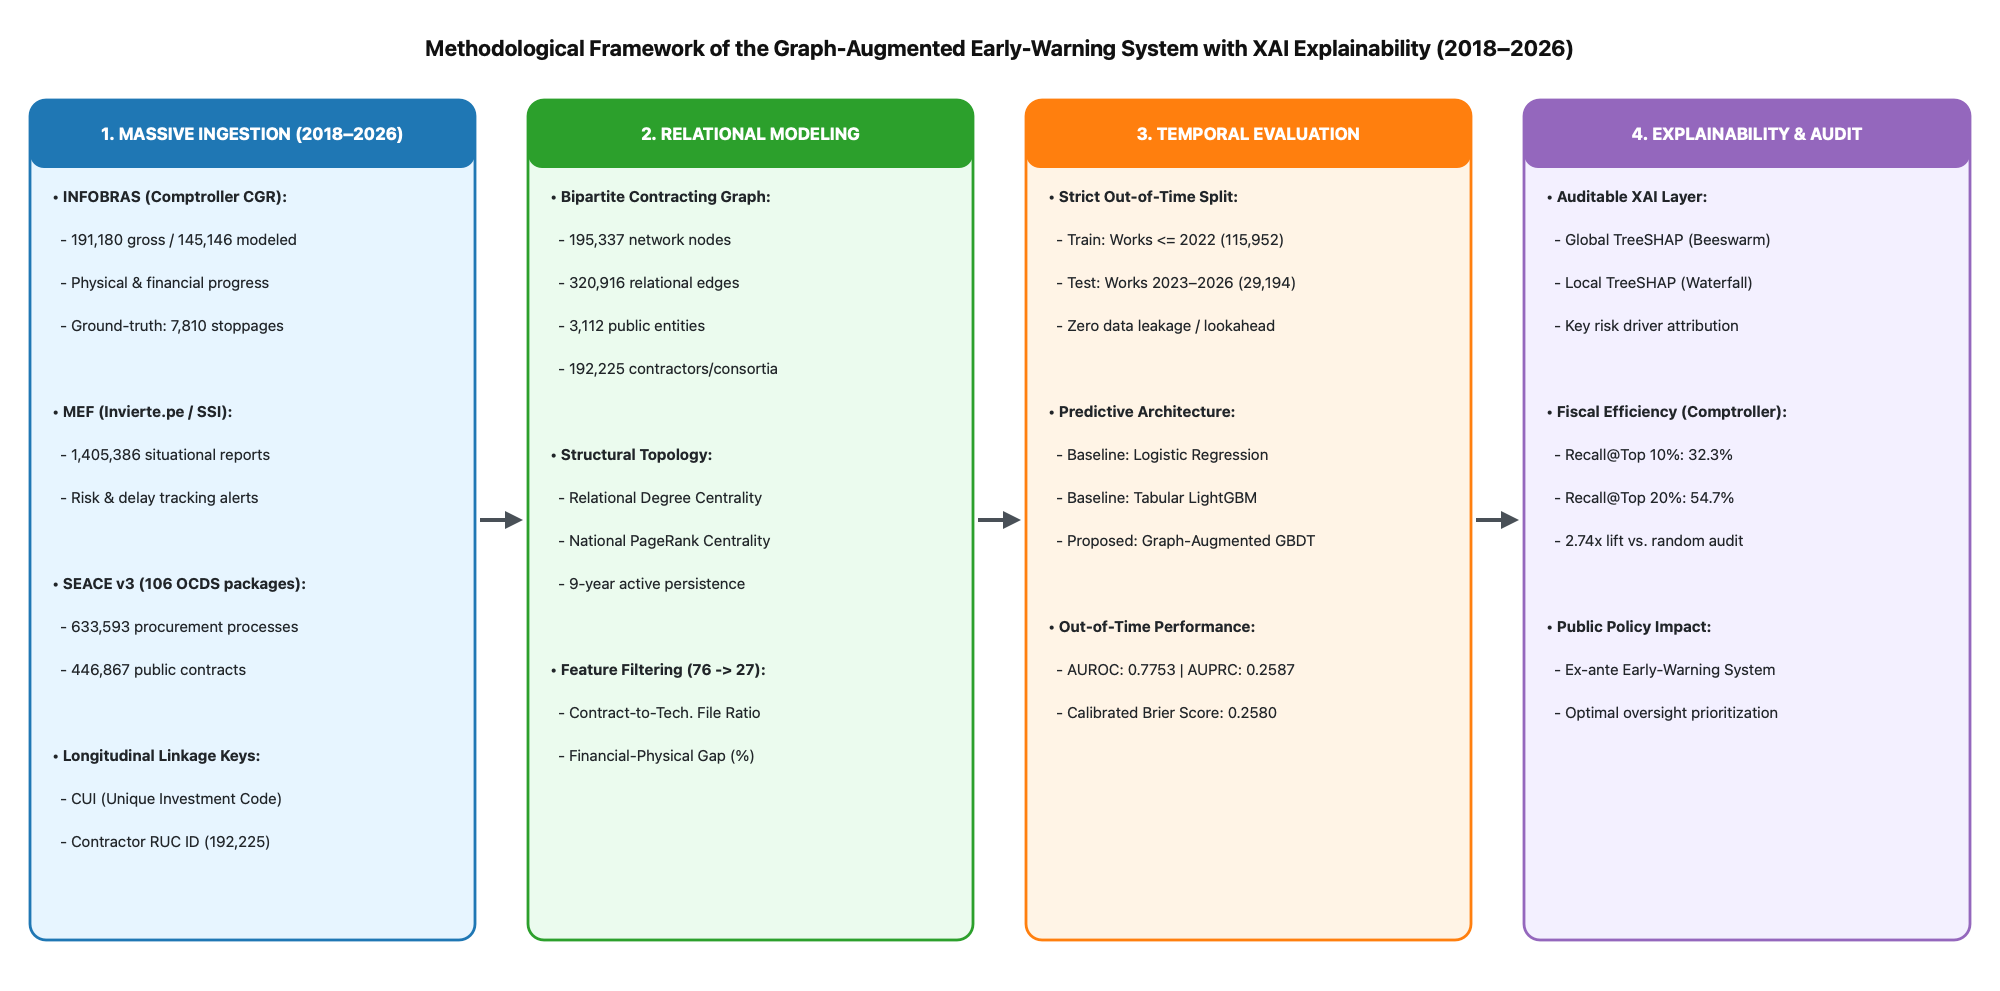
\includegraphics[width=15cm]{figures/fig1_methodological_framework.png}
    \caption{Methodological workflow of the graph-augmented early-warning system: multi-source data ingestion, bipartite contracting graph modeling, prospective out-of-time evaluation, and TreeSHAP explainability layer. Source: Author.}
    \label{fig:framework}
\end{figure}

\subsection*{Bipartite contracting graph modeling and network centralities}
Public procurement interactions are formulated as a dynamic bipartite graph $\mathcal{G} = (\mathcal{V}_E, \mathcal{V}_C, \mathcal{E})$, where $\mathcal{V}_E$ denotes the set of public procuring entities (municipalities, regional governments, ministries; $|\mathcal{V}_E| = 3,112$), $\mathcal{V}_C$ denotes private contractors and consortia ($|\mathcal{V}_C| = 192,225$), and an undirected edge $e_{uv} \in \mathcal{E}$ indicates that entity $u$ awarded a contract to supplier $v$. The resulting graph comprises $|\mathcal{V}| = 195,337$ nodes and $|\mathcal{E}| = 320,916$ relational contracting edges across the nine-year corpus.

For each contractor node $v \in \mathcal{V}_C$, we compute two structural network properties: relational degree centrality ($k_v$), defined as the total number of distinct public buying entities contracting supplier $v$ (Equation 1), and structural PageRank centrality ($PR(v)$), computed via random-walk stationary probability distributions (Equation 2) \citep{page1999pagerank, newman2003structure}:
\begin{equation}
    k_v = \sum_{u \in \mathcal{V}_E} \mathbb{I}((u, v) \in \mathcal{E})
\end{equation}
\begin{equation}
    PR(v) = \frac{1 - d}{|\mathcal{V}|} + d \sum_{u \in \mathcal{N}(v)} \frac{PR(u)}{k_u}
\end{equation}
with damping factor $d = 0.85$.

\subsection*{Domain feature engineering and engineering discrepancy ratios}
An initial candidate feature space of $76$ analytical variables was designed to capture operational friction, contractor multi-year capacity, and physical-financial discrepancies across the linked registries. Following collinearity filtering (Spearman rank correlation threshold $|r| > 0.85$) and the removal of near-zero-variance attributes computed strictly within the historical training partition ($\le 2022$), exactly $27$ explanatory variables ($20$ tabular engineering, financial, and MEF situational tracking indicators plus $7$ SEACE bipartite contracting network features) were retained for predictive modeling and TreeSHAP decomposition. Key domain constructs include:
\begin{itemize}
    \item \textbf{Contract-to-Technical File Ratio ($\rho_i$):} Defined as the contracted amount divided by the approved technical file reference cost ($C_{\text{ET}}$), alongside the absolute budget discrepancy in Peruvian Soles (PEN). Ratios $\rho_i < 0.90$ reflect aggressive bidding discounts, whereas $\rho_i > 1.10$ indicate pre-award cost escalations.
    \item \textbf{Financial-Physical Gap ($\Delta_{\text{fin-phys}}$):} Computed as the percentage difference between cumulative financial execution and certified physical progress on site. Positive gaps identify premature capital disbursement relative to verified physical delivery.
    \item \textbf{Physical Schedule Lag ($\Delta_{\text{sched}}$):} Percentage gap between scheduled physical progress and actual certified physical progress achieved on site.
    \item \textbf{Problem Report Ratio ($\theta_{\text{prob}}$):} The proportion of monthly situational tracking reports in MEF Invierte.pe flagged with operational, financial, or legal execution problems, complemented by MEF risk alerts and total situational reports.
\end{itemize}

\subsection*{Prospective out-of-time validation and cost-sensitive learning}
From the $191,180$ gross public works recorded in INFOBRAS ($7,962$ stalled records; $4.16\%$ gross prevalence), $46,034$ administrative records corresponding to interventions lacking a valid start date outside the $2012$--$2026$ window, projects remaining in preparatory acts without initiated physical execution, or duplicate/voided entries were excluded. This filtering established the final analytical cohort of $N = 145,146$ modeled public works containing $7,810$ verified stalled projects ($5.38\%$ of the analytical panel, equivalent to $4.16\%$ of the gross registry). To strictly prevent lookahead bias, chronological partitioning was enforced: the training cohort comprises $115,952$ public works initiated on or before $2022$ ($5,027$ stalled works; $4.34\%$ rate), while the blind prospective test cohort comprises $29,194$ works initiated between $2023$ and $2026$ ($2,783$ stalled works; $9.53\%$ rate). Cost-sensitive weighted cross-entropy loss was optimized via LightGBM \citep{ke2017lightgbm} with positive class weighting $w_1 = 21.9$ to address class imbalance without synthetic oversampling artifacts.

\section*{Experimental results and analysis}

\subsection*{Prospective out-of-time benchmarking}
Table 1 summarizes prospective performance across the $29,194$ test works initiated between $2023$ and $2026$. The proposed Graph-Augmented LightGBM model achieves an AUROC of $0.7753$ and an AUPRC of $0.2587$, outperforming balanced logistic regression by over $10.5$ AUROC points ($0.7753$ vs. $0.6695$) and demonstrating superior probability calibration with a Brier score of $0.2580$ (Figure 2).

Comparing the Graph-Augmented LightGBM architecture against the purely tabular LightGBM baseline (Table 1) reveals two operationally critical insights regarding the contribution of the bipartite contracting network. First, while on-site physical execution metrics naturally dominate global splits once a project is well underway, the bipartite graph topological features (contractor structural PageRank, relational degree centrality, and multi-entity dispersion) provide their decisive discriminative lift during early contract stages---when certified physical progress remains near zero---and in the extreme upper tail of risk prioritization. Specifically, incorporating network topology elevates early stoppage capture in the highest-priority audit brackets from $16.53\%$ to $17.25\%$ in $\text{Recall@Top5\%}$ ($+0.72$ percentage points) and from $31.62\%$ to $32.27\%$ in $\text{Recall@Top10\%}$ ($+0.65$ percentage points), allowing oversight teams to detect additional high-value stalled projects under tight inspection budgets. Second, relational contracting features substantially improve out-of-time probability calibration across the prospective test horizon, reducing the Brier score from $0.2652$ (tabular baseline) to $0.2580$ (proposed model) by penalizing overextended contractors operating simultaneously across multiple procuring jurisdictions.

\begin{table}[htbp]
\centering
\caption{Prospective Out-of-Time Performance Comparison on Peruvian Public Works (2023--2026). Source: Author.}
\label{tab:benchmarks}
\small
\begin{tabular*}{\textwidth}{@{\extracolsep{\fill}}lcccccc@{}}
\toprule
\textbf{Model Architecture} & \textbf{AUPRC} & \textbf{AUROC} & \textbf{Brier Score} & \textbf{Rec@Top5\%} & \textbf{Rec@Top10\%} & \textbf{Rec@Top20\%} \\
\midrule
1. Balanced Logistic Regression & 0.1567 & 0.6695 & 0.3196 & 9.67\% & 19.94\% & 36.26\% \\
2. LightGBM (Tabular Baseline)  & 0.2550 & 0.7733 & 0.2652 & 16.53\% & 31.62\% & 54.37\% \\
3. \textbf{LightGBM + Graph Network (Proposed)} & \textbf{0.2587} & \textbf{0.7753} & \textbf{0.2580} & \textbf{17.25\%} & \textbf{32.27\%} & \textbf{54.65\%} \\
\bottomrule
\end{tabular*}
\end{table}

\begin{figure}[htbp]
    \centering
    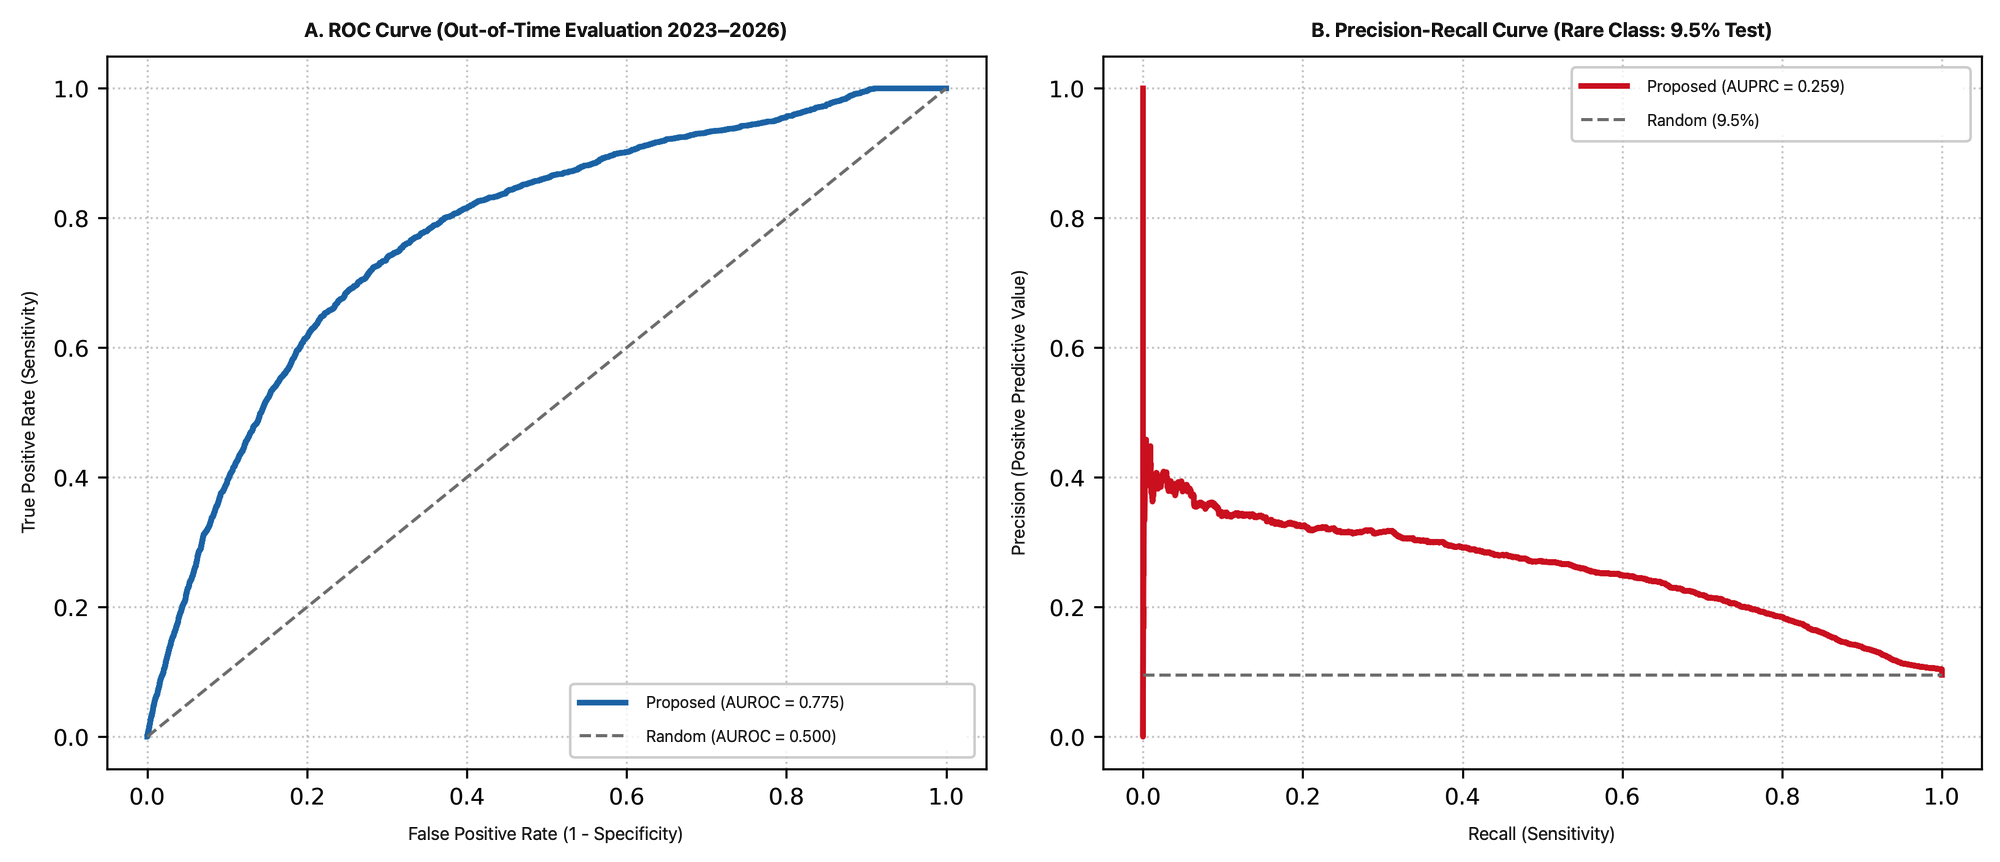
\includegraphics[width=15cm]{figures/fig2_roc_pr_curves.png}
    \caption{Prospective out-of-time evaluation curves (2023--2026): (A) Receiver Operating Characteristic (AUROC = 0.775); (B) Precision-Recall curve (AUPRC = 0.259) against the 9.53\% test baseline. Source: Author.}
    \label{fig:curves}
\end{figure}

\subsection*{Fiscal audit efficiency and resource allocation optimization}
For institutional audit authorities constrained by finite inspectorate resources, Figure 3 illustrates the cumulative audit capture curve. Prioritizing technical audits on the top $10\%$ highest-risk projects captures $32.27\%$ of all stalled works across the national territory. Expanding the audit inspection budget to the top $20\%$ captures $54.65\%$ of all stalled public works nationwide. This corresponds to an empirical efficiency multiplier of $2.74\times$ over uniform or random inspection strategies, directly safeguarding public capital.

\begin{figure}[htbp]
    \centering
    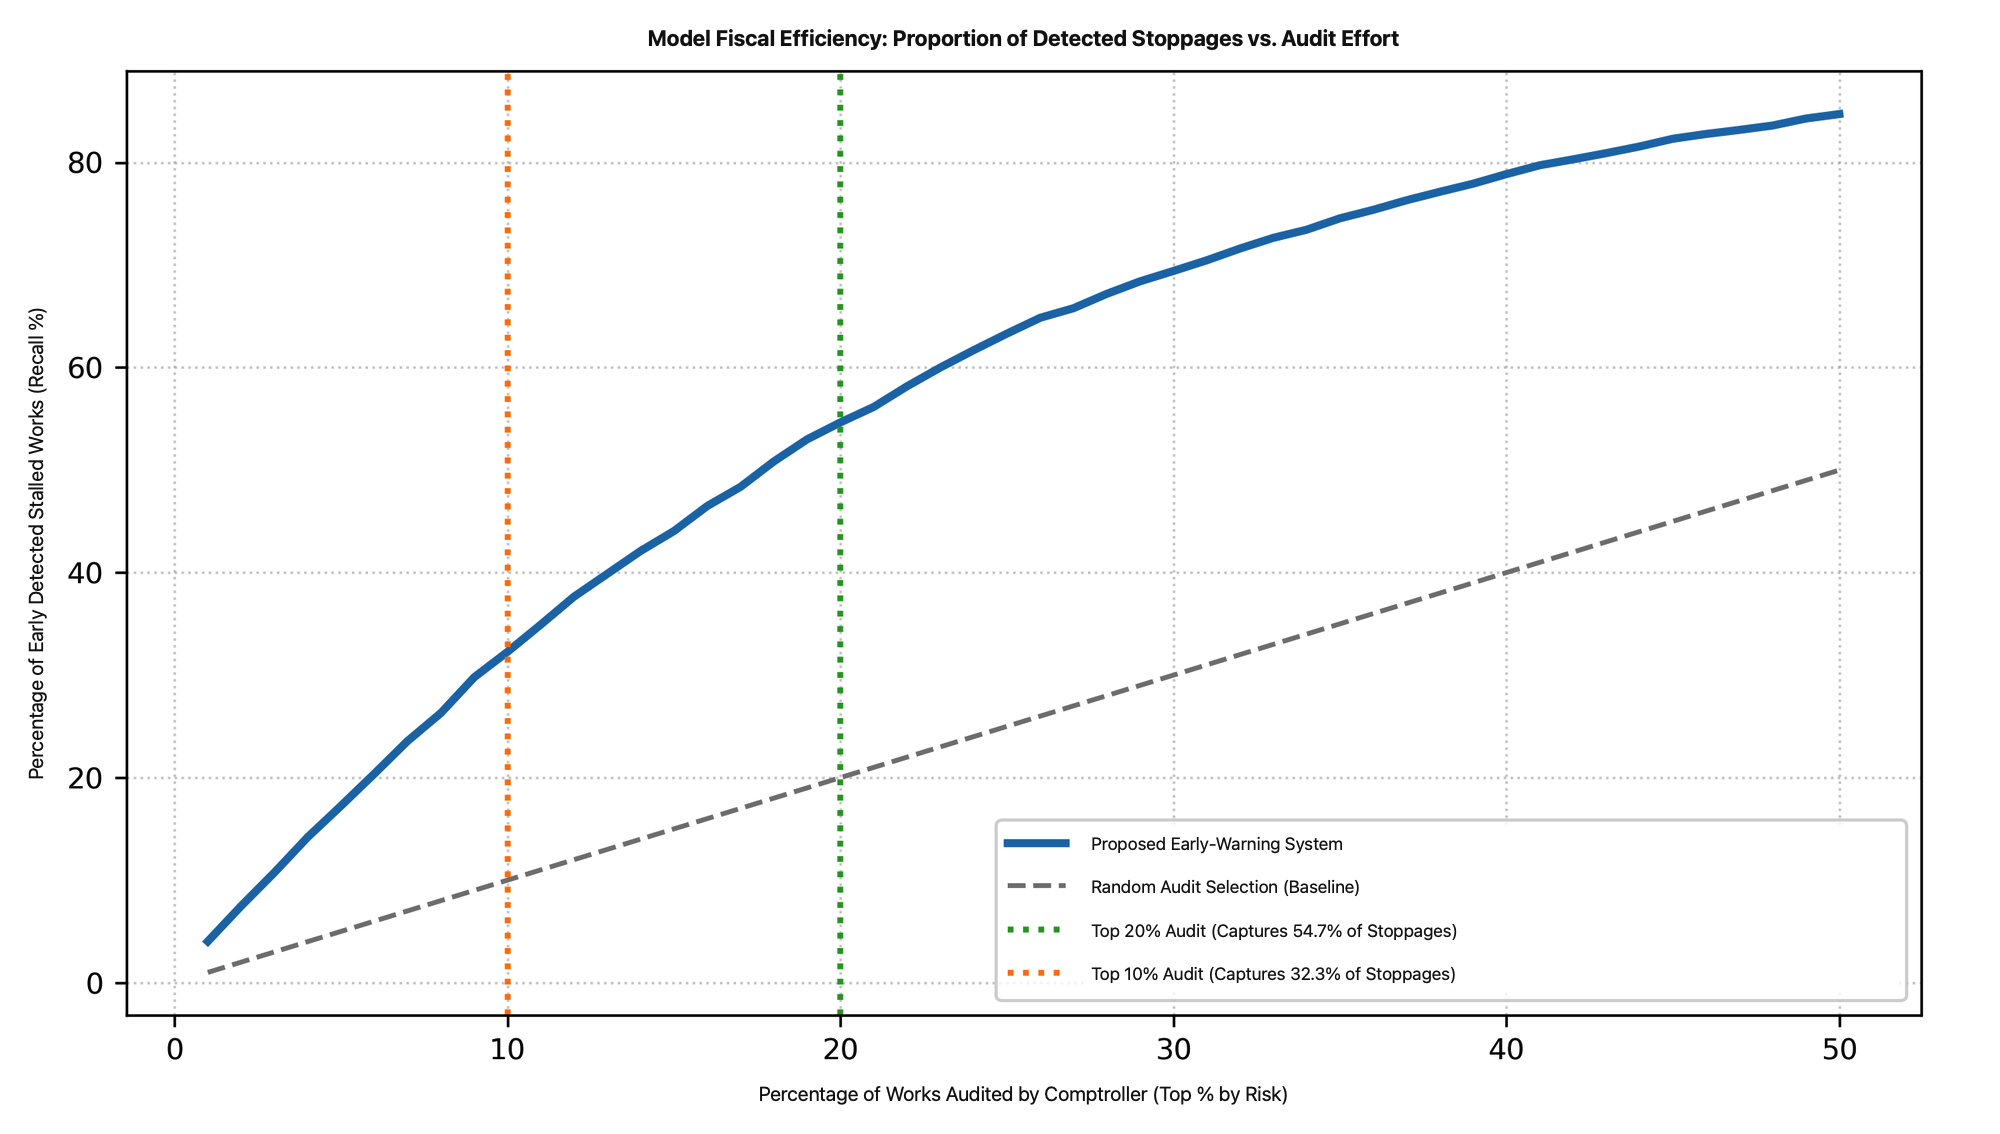
\includegraphics[width=13.5cm]{figures/fig5_audit_efficiency_recall_curve.png}
    \caption{Cumulative audit efficiency curve: percentage of stalled infrastructure projects detected across Peru as a function of allocated technical audit inspection budget. Source: Author.}
    \label{fig:audit}
\end{figure}

\subsection*{Explainability and case auditability via TreeSHAP}
TreeSHAP global attribution across $3,000$ prospective test cases (Figure 4) decomposes the directional impact of the $27$ retained features ($14$ top individual drivers plus the aggregated impact of the remaining $13$ features). Certified actual physical progress, financial-physical execution gaps ($\Delta_{\text{fin-phys}}$), financial execution levels, MEF tracking registration, problem report ratios ($\theta_{\text{prob}}$), MEF risk alerts, and physical schedule lag ($\Delta_{\text{sched}}$) emerge as the dominant global predictors of work stoppage.

Figure 5 reconstructs an individual explainable audit dossier for a real stalled public infrastructure project from the prospective test set (reference cost of $\text{S/ } 108,582,317$ and budget discrepancy of $\text{S/ } 12,027,324$). Starting from the population baseline log-odds of $E[f(X)] = -2.352$, the cumulative additive contributions of the project's risk factors drive the final model output to $f(x) = +2.393$, which corresponds via the logistic sigmoid link $\sigma(f(x)) = (1 + e^{-2.393})^{-1}$ to a predicted stoppage probability of $91.6\%$. Specifically, the prediction is propelled upward by an incomplete actual physical progress stagnating at $69.27\%$ ($+2.47$ log-odds), a synchronized financial-physical execution profile ($0.00\%$ gap at $69.27\%$ financial execution; $+0.41$ and $+0.14$ log-odds), a high MEF problem report ratio of $0.50$ across $3$ situational reports ($+0.40$ and $+0.08$ log-odds), an accumulated physical schedule lag of $19.47\%$ behind the contractual baseline ($+0.37$ log-odds), active MEF tracking registration ($+0.23$ log-odds), a substantial absolute budget discrepancy of $\text{S/ } 12,027,324$ ($+0.20$ log-odds), project scale ($\text{S/ } 108,582,317$; $+0.12$ log-odds), and $+0.19$ log-odds from the remaining $18$ features.

\begin{figure}[htbp]
    \centering
    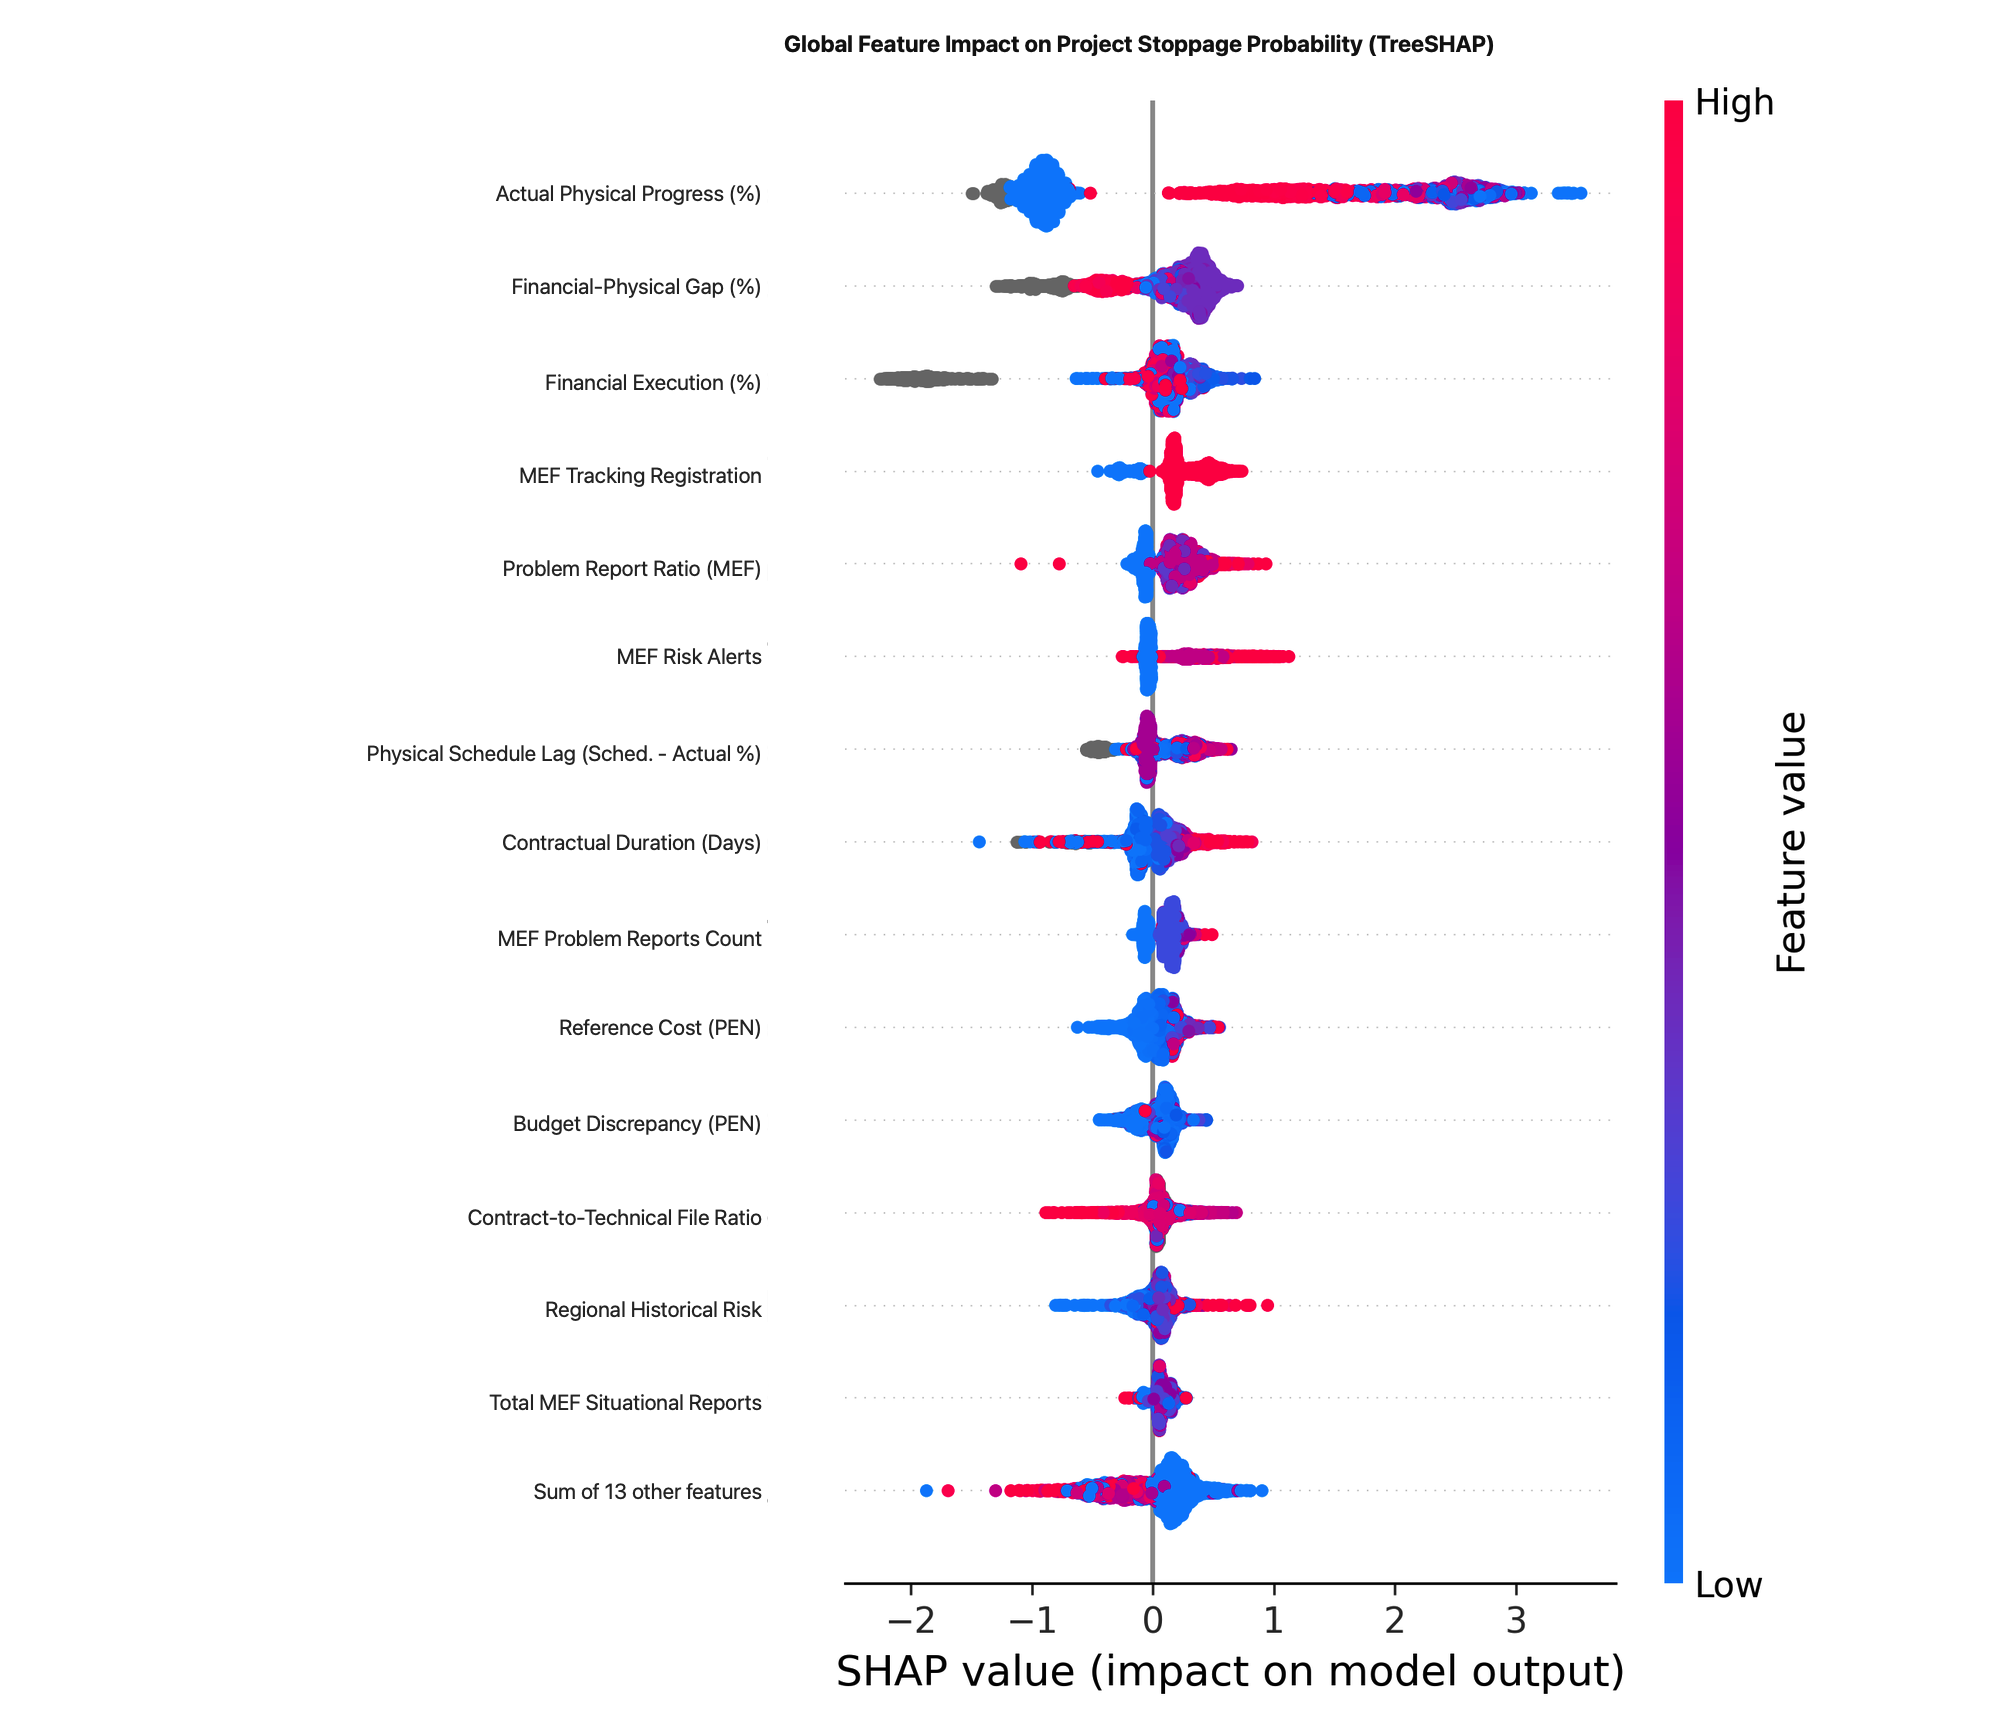
\includegraphics[width=14.5cm]{figures/fig3_shap_summary_beeswarm.png}
    \caption{TreeSHAP global feature summary beeswarm plot displaying directional impact and importance ranking of the 27 retained risk drivers (top 14 individual features plus 13 aggregated features) on project stoppage probability. Source: Author.}
    \label{fig:beeswarm}
\end{figure}

\begin{figure}[htbp]
    \centering
    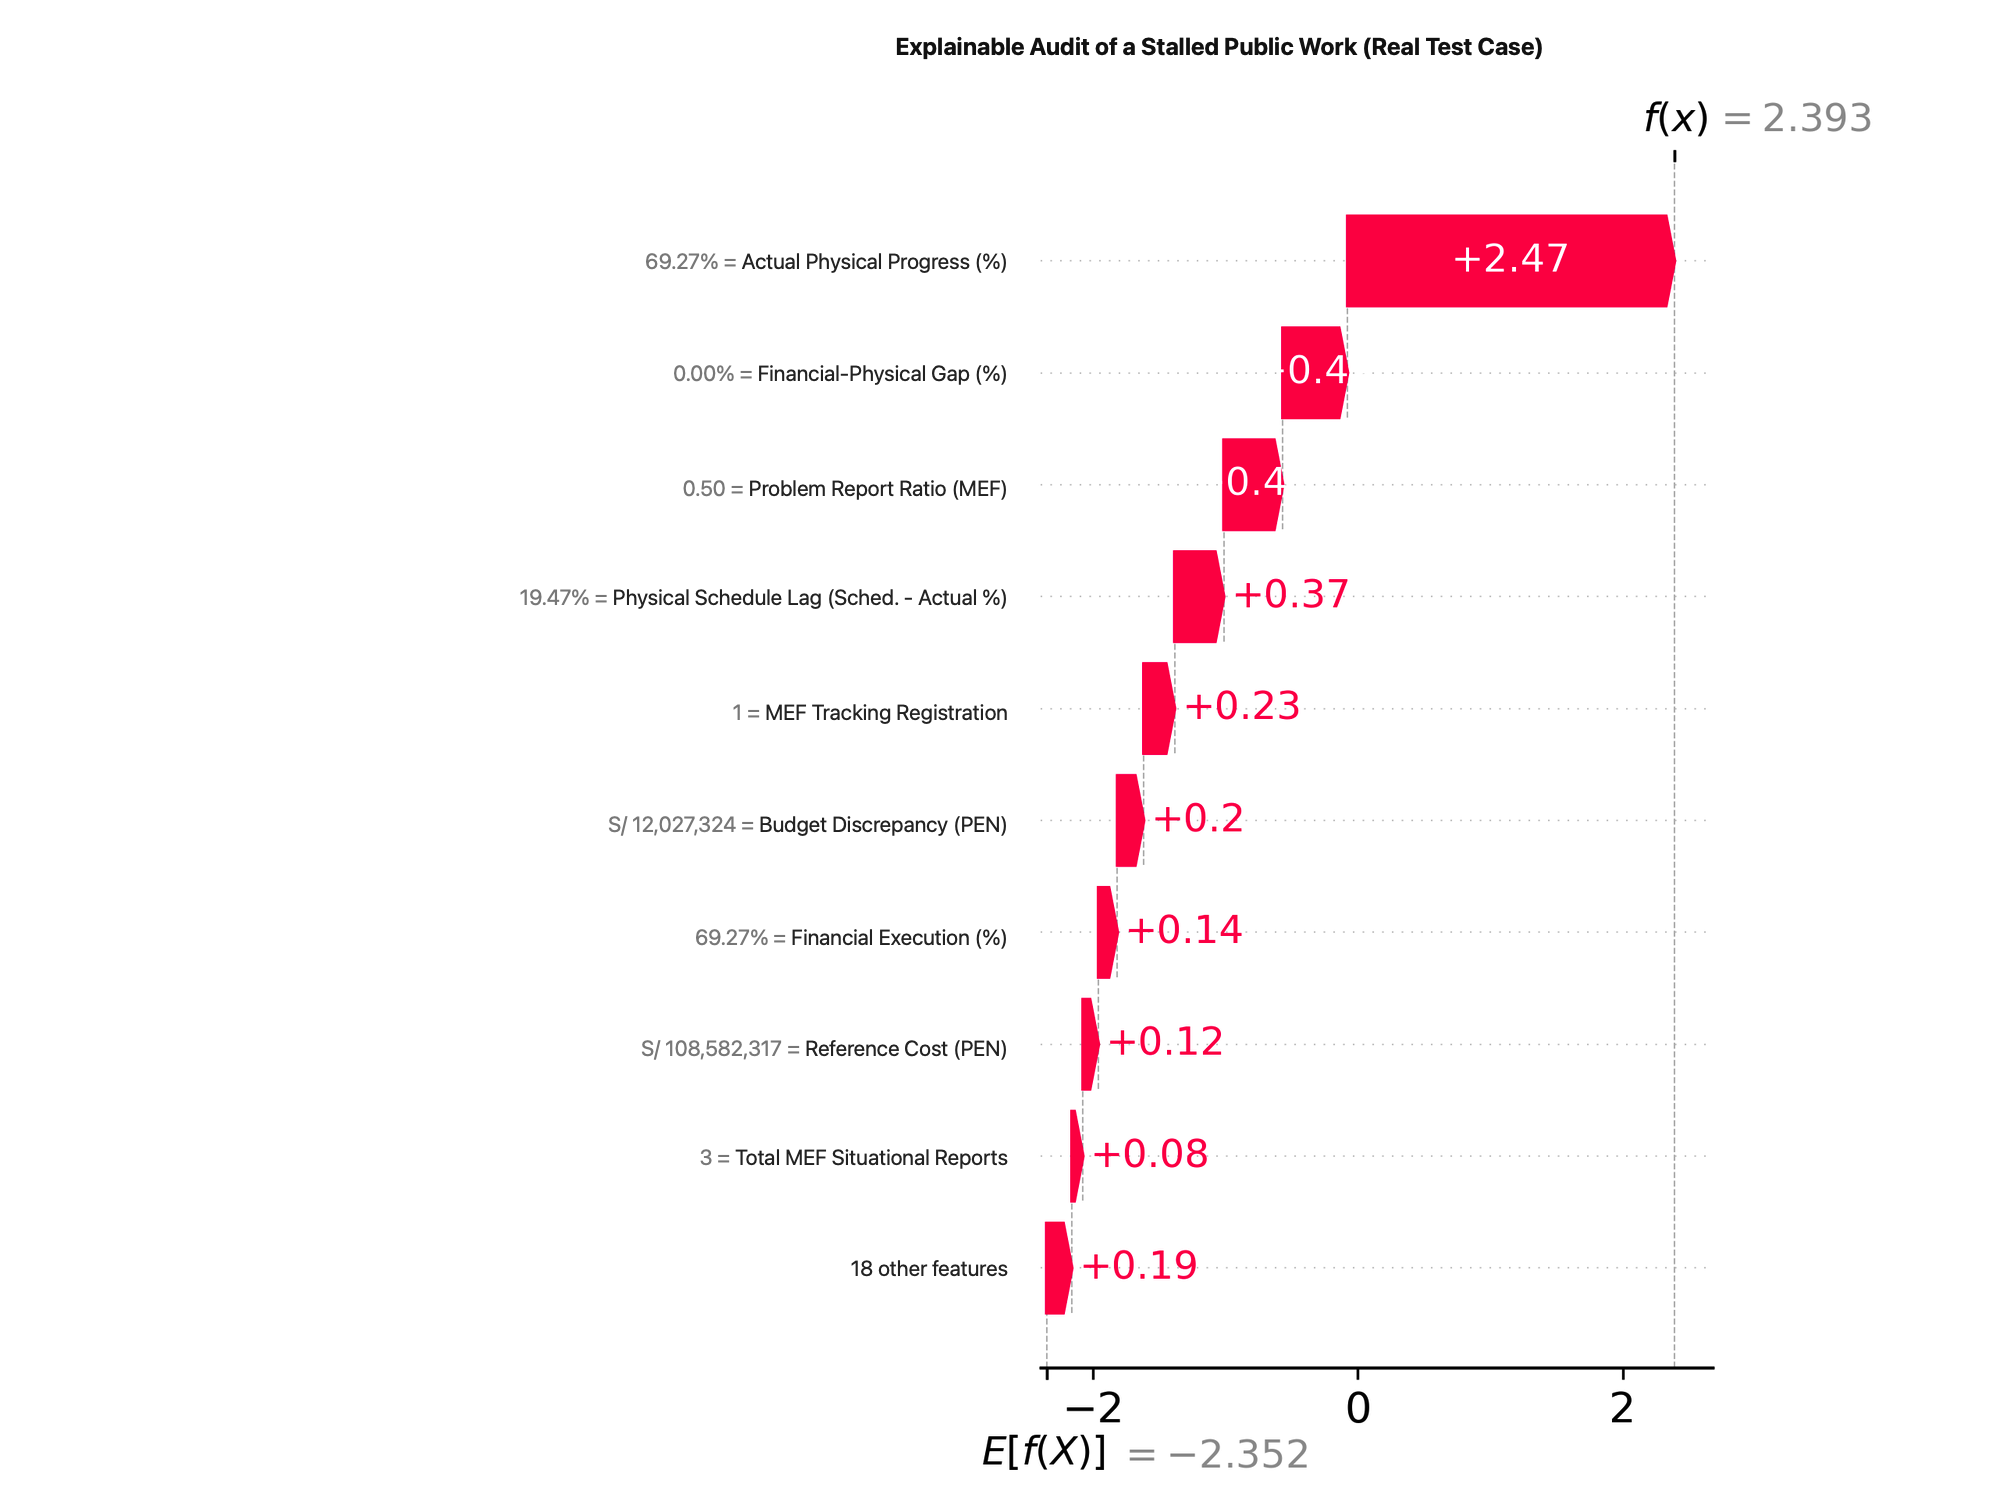
\includegraphics[width=14.5cm]{figures/fig4_shap_waterfall_auditing_case.png}
    \caption{Local TreeSHAP waterfall audit reconstruction for a real stalled infrastructure project in the prospective test set ($E[f(X)] = -2.352$ to $f(x) = +2.393$, or $91.6\%$ stoppage probability), isolating line-item evidentiary attribution for oversight teams. Source: Author.}
    \label{fig:waterfall}
\end{figure}

\section*{Conclusions and comments}
The main conclusions and comments of this study are summarized as follows:
\begin{enumerate}
    \item Integrating nationwide procurement networks (SEACE v3) with longitudinal physical progress tracking (INFOBRAS and MEF Invierte.pe) across an analytical cohort of $N = 145,146$ modeled works (filtered from $191,180$ gross records) enables the construction of an auditable early-warning system that significantly outperforms traditional non-relational construction management models, achieving an AUROC of $0.7753$ and an AUPRC of $0.2587$ under strict prospective out-of-time evaluation.
    \item Bipartite contracting graph modeling ($195,337$ nodes, $320,916$ edges) demonstrates that contractor structural topology---specifically degree centrality, PageRank, and multi-year market presence---provides critical early-stage discriminatory lift ($\text{Recall@Top5\%}$ rising from $16.53\%$ to $17.25\%$) and superior probability calibration (Brier score reduced from $0.2652$ to $0.2580$), penalizing overcommitted construction firms operating across fragmented jurisdictions.
    \item From a public policy and fiscal efficiency perspective, auditing merely the top $20\%$ highest-risk projects flagged by the model captures $54.65\%$ of all stalled public works nationwide, representing a $2.74\times$ efficiency multiplier over uniform or random inspection methods for Supreme Audit Institutions.
    \item TreeSHAP explainability across the $27$ retained explanatory features bridges the gap between predictive artificial intelligence and legal audit defense, decomposing predictions into line-item engineering evidentiary dossiers that quantify physical schedule lags ($19.47\%$), stagnant execution ($69.27\%$), and million-soles budget discrepancies prior to formal site abandonment.
    \item The framework provides an open-source, scalable blueprint for construction procurement authorities in emerging economies to transition from reactive ex-post forensic accounting to proactive, preventive contract governance.
\end{enumerate}

\noindent\textbf{Author contributions:} J.M.V.C.: Conceptualization, methodology, software, computational graph architecture, SEACE/INFOBRAS/MEF data curation, formal analysis, validation, investigation, visualization, and manuscript writing---original draft preparation, review, and editing. The author has read and agreed to the published version of the manuscript.
\vspace{0.2cm}

\noindent\textbf{Funding:} This research received no external funding.
\vspace{0.2cm}

\noindent\textbf{Acknowledgments:} The author expresses gratitude to the open-data initiatives of the Contralor{\'\i}a General de la Rep{\'u}blica (INFOBRAS), Ministerio de Econom{\'\i}a y Finanzas (Invierte.pe), and OECE (SEACE) for making administrative public procurement datasets accessible for scientific research.
\vspace{0.2cm}

\noindent\textbf{Conflicts of interest:} The author declares no conflict of interest.

\bibliographystyle{plainnat}
\bibliography{references}

\end{document}
